\documentclass{beamer}

\mode<presentation>{
  \usetheme{Warsaw}
  % \usetheme{Montpellier}
  \setbeamercovered{transparent}
}

\usepackage[french]{babel}
\usepackage[latin1]{inputenc}
\usepackage{times}
\usepackage[T1]{fontenc}
\usepackage{subfigure}

\usepackage{algorithm}
\usepackage{algorithmic}

%%%%%%%%%%%%%%%%%%%%%%%%%%%%%%%%%%%%%%%%%%%%%%%%%%%%%%%%%%%% 
\title{Projet PROMAIN}
\subtitle{Architecture des noeuds de t�l�op�ration de la main robot}

\author{Nizar ABAK-KALI}

\institute{
  PARIS 8 Saint-Denis \\
  \tiny{nabak-kali@etud.univ-paris8.fr} 
}

\date{\today}


\pgfdeclareimage[height=0.8cm]{le-logo}{liasd}
\logo{\pgfuseimage{le-logo}}

\AtBeginSection[]{
  \begin{frame}<beamer>{PLAN DE LA PRESENTATION}
    \tableofcontents[currentsection]
  \end{frame}
}

%%%%%%%%%%%%%%%%%%%%%%%%%%%%%%%%%%%%%%%%%%%%%%%%%%%%%%%%%%%% 
\begin{document}

\begin{frame}
  \titlepage
\end{frame}

\begin{frame}{PLAN DE LA PRESENTATION}
  \tableofcontents
\end{frame}

%%%%%%%%%%%%%%%%%%%%%%%%%%%%%%%%%%%%%%%%%%%%%%%%%%%%%%%%%%%% 
\section{Introduction}

%%%%%%%%%%%%% ETAT DES LIEUX
\begin{frame}
  \begin{exampleblock}{Solution existante (Projet Universit� Rennes)}
    \begin{figure}[!t]
      T�l�op�ration de main robotique. \\
      \subfigure[de dos]{\includegraphics[scale=0.1]{figure/InMoovhand.jpg}}\quad
      \subfigure[de face]{\includegraphics[scale=0.080]{figure/main_de_face.JPG}}\quad
      \caption{InMoovhand version 2012}
      \label{fig1}
    \end{figure}
  \end{exampleblock}
\end{frame}
%%%%%%%%%%%%%%% Problematique rencontre
\begin{frame}
  \begin{alertblock}{Probl�matique rencontr�e}
    \begin{itemize}
    \item Contr{\^o}le d'un servo-moteur avec ROS.
    \item Connexion de la InMoovhand avec ROS ou PC ou carte embarqu�e.
    \item Choix du servo-moteur : classique ou s�rie (\emph{c.f.} Dynamixel).
    \item Solution Arduino ou carte embarqu�e alternative.
    \end{itemize}
  \end{alertblock}
\end{frame}

%%%%%%%%%%%%%%%%%%%%%%%%%%%%%%%%%%%%%%%%%%%%%%%%%%%%%%%%%%%% 
\section{Contr{\^o}le de Servo-moteur}

\begin{frame}
  \begin{exampleblock}{Outils : RoS Hydro}

    \begin{columns}

      \begin{column}{.50\textwidth}
        \begin{figure}[!t]
          \includegraphics[scale=0.1]{figure/Hydromedusa.jpg}
          \label{fig-hydro}
        \end{figure}
      \end{column}

      \hfill%
      \begin{column}{.50\textwidth}
        \begin{itemize}
        \item ROS: Syst�me d'exploitation pour contr{\^o}ler des robots .
        \item rosserial-arduino: Package de ROS pour contr{\^o}ler une carte embarqu�e arduino.
        \end{itemize}
      \end{column}%
    \end{columns}

  \end{exampleblock}

\end{frame}


\begin{frame}
  \begin{exampleblock}{Outils : Arduino Uno}
    \begin{columns}

      \begin{column}{.40\textwidth}
        \begin{figure}[!t]
          \includegraphics[scale=1.0]{figure/ArduinoUno.jpg}
          \label{fig-arduino}
        \end{figure}
      \end{column}

      \hfill%
      \begin{column}{.60\textwidth}
        \begin{itemize}
        \item Prix bas : environ 20 euros.
        \item Alimentation : 5V pour l'alimentation (par usb), 7-12V recommand�.
        \item Nombres de servo-moteur maximum : 6.
        \end{itemize}
      \end{column}%
    \end{columns}
  \end{exampleblock}
\end{frame}

\begin{frame}
  \begin{exampleblock}{Schema pratique: }
    \begin{columns}
      \begin{column}{.50\textwidth}
        \begin{figure}[!t]
          \includegraphics[scale=0.1]{figure/arduino_servo.png}
          \label{fig-arduino-servo}
        \end{figure}
      \end{column}
      \hfill%
      \begin{column}{.73\textwidth}
        \begin{itemize}
        \item contr{\^o}le depuis ROS.
        \item Instructions re�ues par port usb.
        \item Signaux transmits au Servo-moteur branch�.
        \end{itemize}
      \end{column}%
    \end{columns}
  \end{exampleblock}

\end{frame}

%%%%%%%%%%%%%%%%%%%%%%%%%%%%%%%%%%%%%%%%%%%%%%%%%%%%%%%%%%%% 
\section{Connexion de la main robot InMoovhand}

\begin{frame}
  % \textbf{ La connexion de la main reviens � la connexion de chaque moteur de la main � la carte Arduino }
  \begin{exampleblock}{La connexion de la main revient � la connexion de chaque moteur de la main � la carte Arduino}
    \begin{columns}
      \begin{column}{.25\textwidth}
        \begin{figure}[!t]
          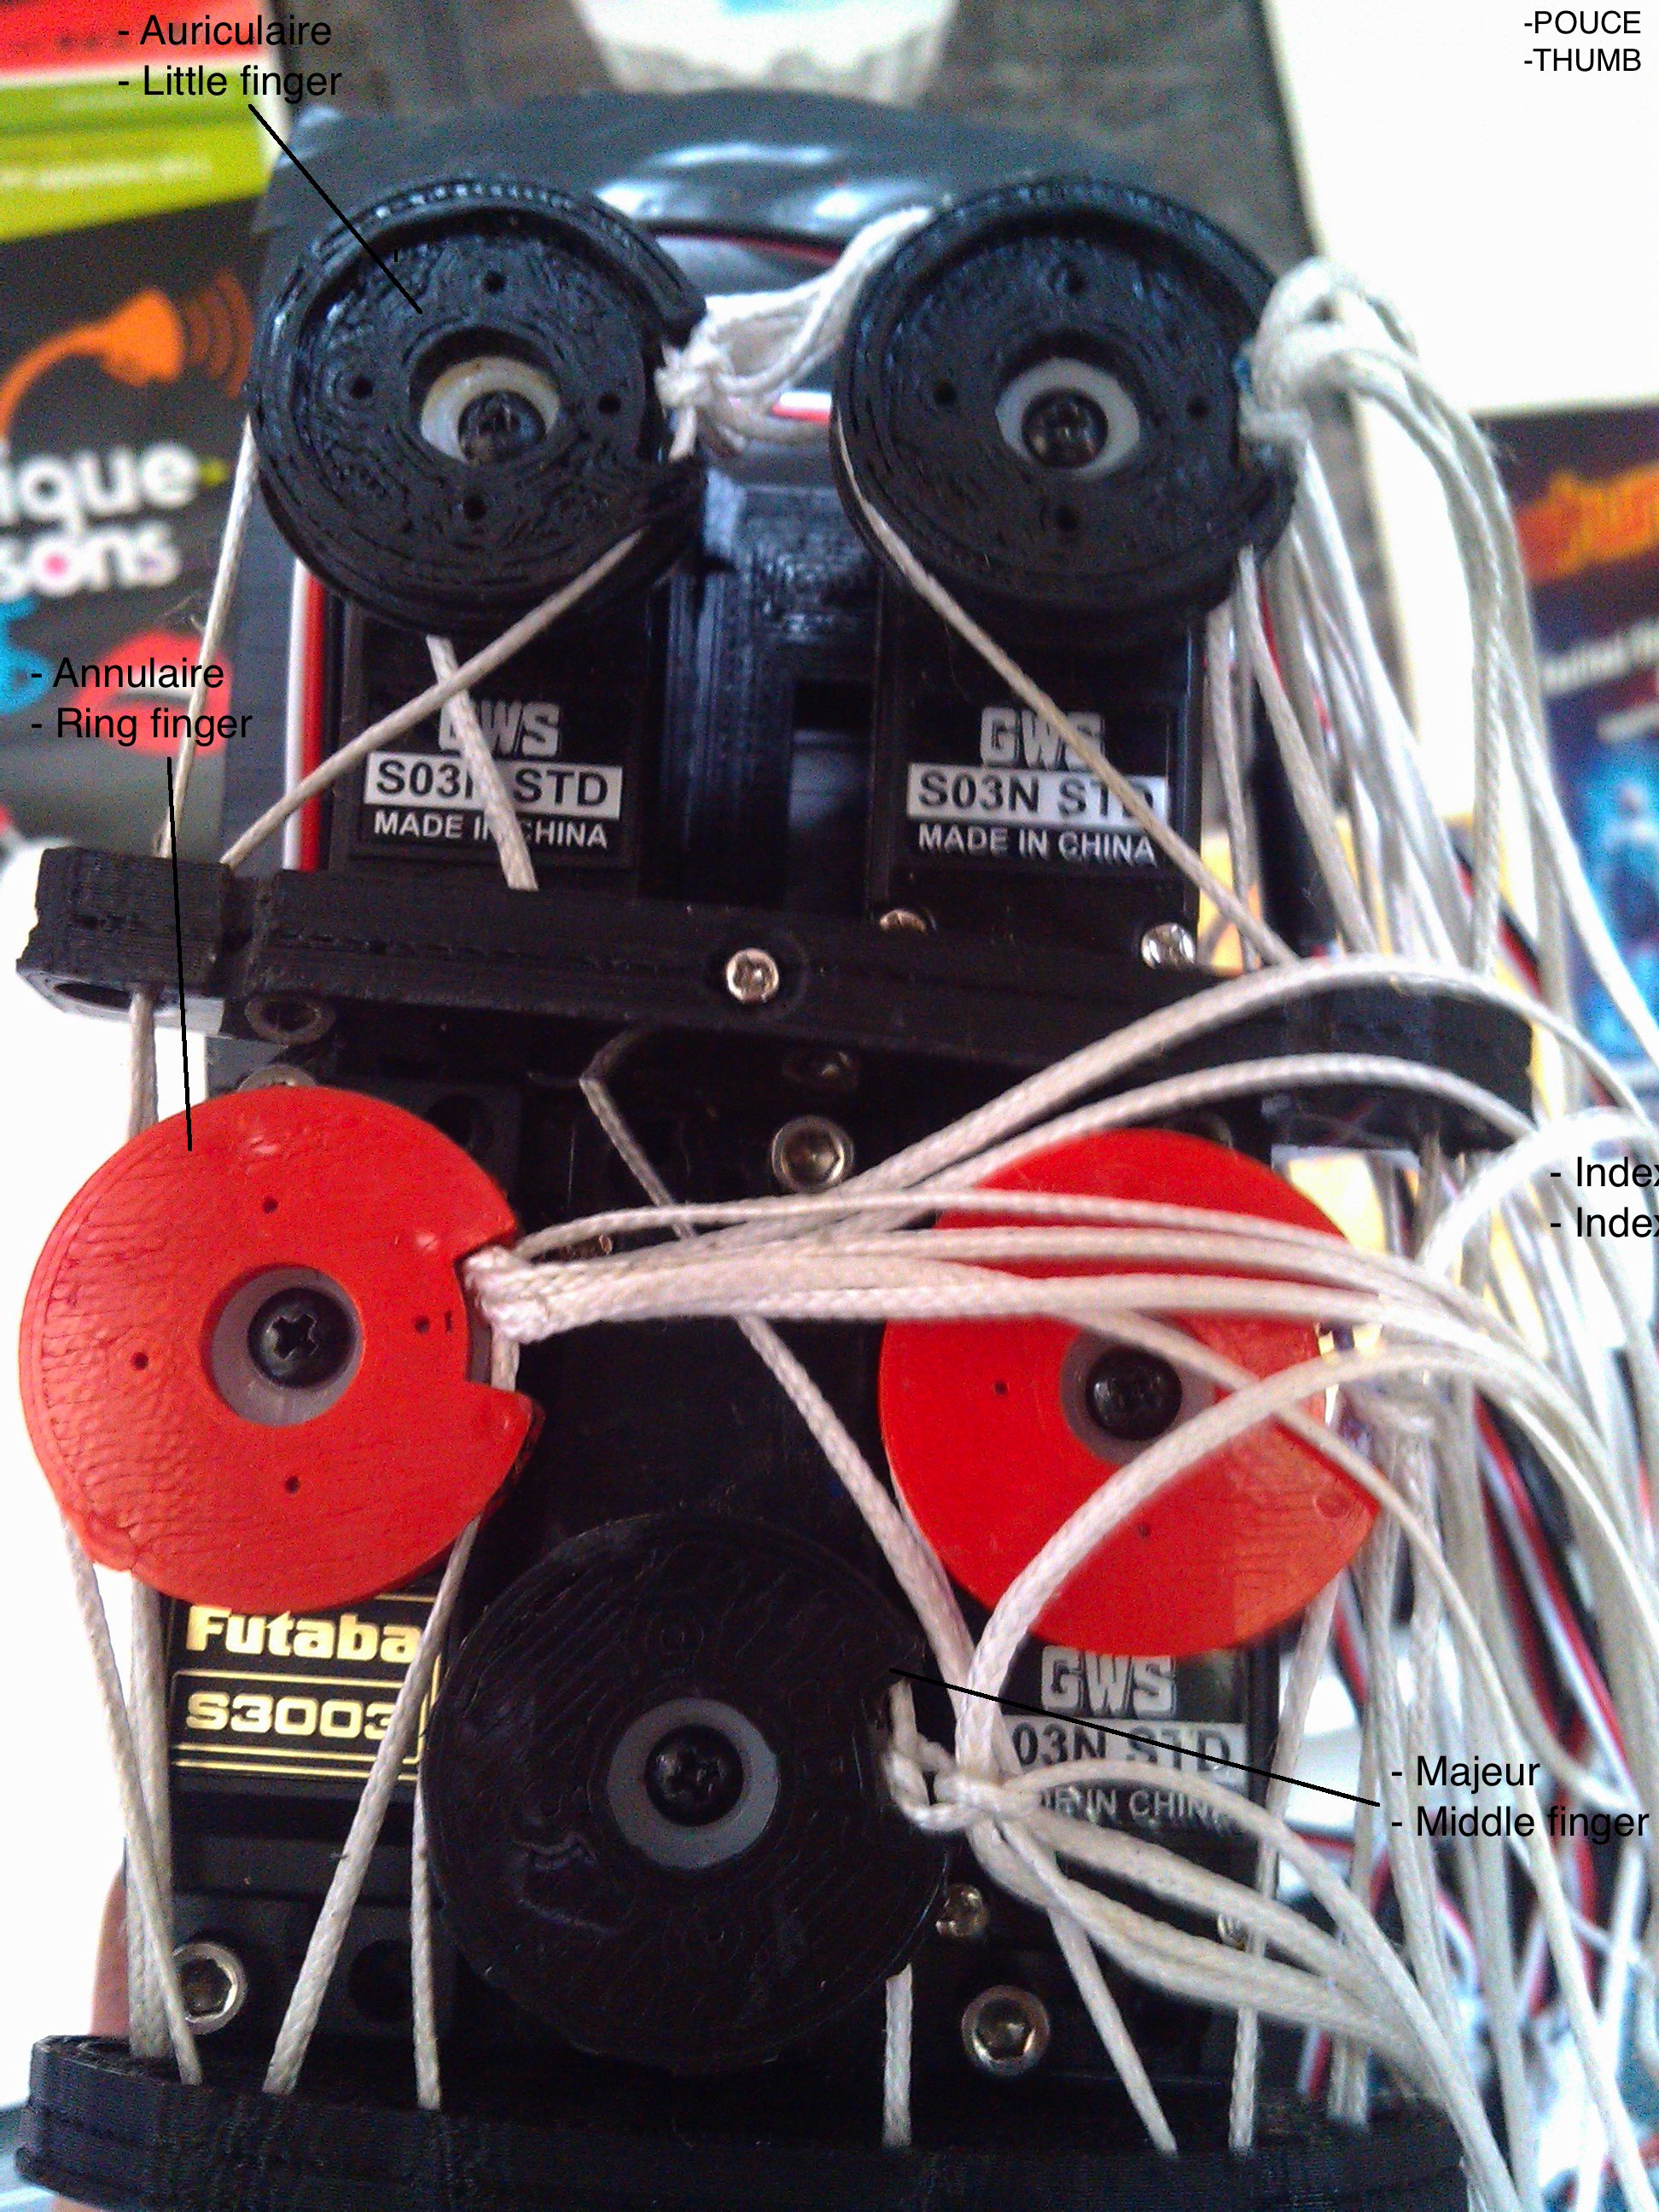
\includegraphics[scale=0.075]{figure/in-moov-servo-moteursbis.png}
          \label{fig-inmoov-servo-motor-bis}
        \end{figure}
      \end{column}
      \hfill%
      \begin{column}{.50\textwidth}
        \begin{itemize}
        \item 1 moteur => 1 commande => 1 IO.
        \item 1 IO = fil jaune de commande.
        \item possibilit� de couplage des alim et des masses?
        \item Amperage max de servomoteurs.
        \end{itemize}
      \end{column}%
    \end{columns}
  \end{exampleblock}
\end{frame}



%%%%%%%%%%%%%%%%%%%%%%%%%%%%%%%%%%%%%%%%%%%%%%%%%%%%%%%%%%%% 
\section{Conclusion}
\begin{frame}
  \begin{exampleblock}{Travail accompli}
    \begin{itemize}
    \item {\'E}tude des paquets ROS arduino.
    \item Prise en main de l'API rosserial-arduino.
    \item Cr�ation d'un premier paquet de t�l�op�ration d'un
      servo-moteur classique.
    \end{itemize}
  \end{exampleblock}
\end{frame} 

\begin{frame}
  \begin{alertblock}{Objetifs}
    \begin{itemize}
    \item contr{\^o}le de plusieurs servo-moteurs. 
    \item contr{\^o}le de plusieurs servo-moteurs serie.
      % \item Couplage des projets  .
    \item Utilisation des r�sultats de ce projet pour le contr{\^o}le
      de la main par cam�ra RGB-D.
    \end{itemize}
  \end{alertblock}
\end{frame}

\begin{frame}
  \titlepage
\end{frame}
%%%%%%%%%%%%%%%%%%%%%%%%%%%%%%%%%%%%%%%%%%%%%%%%%%%%%%%%%%%% 

\end{document}


